À la suite d'une candidature spontanée et de premiers contacts avec Thomas Dudouet et Clément Chastagnol, je me suis entretenu avec Christian Frisch afin de savoir quelle pourrait être ma contribution chez Data Publica. Ayant suivi une formation à l'INSA plutôt orienté big data / data mining, Christian Frisch m'a alors proposé de travailler sur l'une des fonctionnalité du produit C-Radar.

\section{La fonctionnalité de C-Radar} % (fold)
\label{sec:la_fonctionnalite_de_c_radar}
    L'objectif de mon stage serait le suivant : améliorer la fonctionnalité de C-Radar permettant d'être au courant de l'intégralité de la communication des entreprises françaises et belges simplement en s'abonnant à un newsletter.\\

    \begin{figure}[h!]
        \centering
        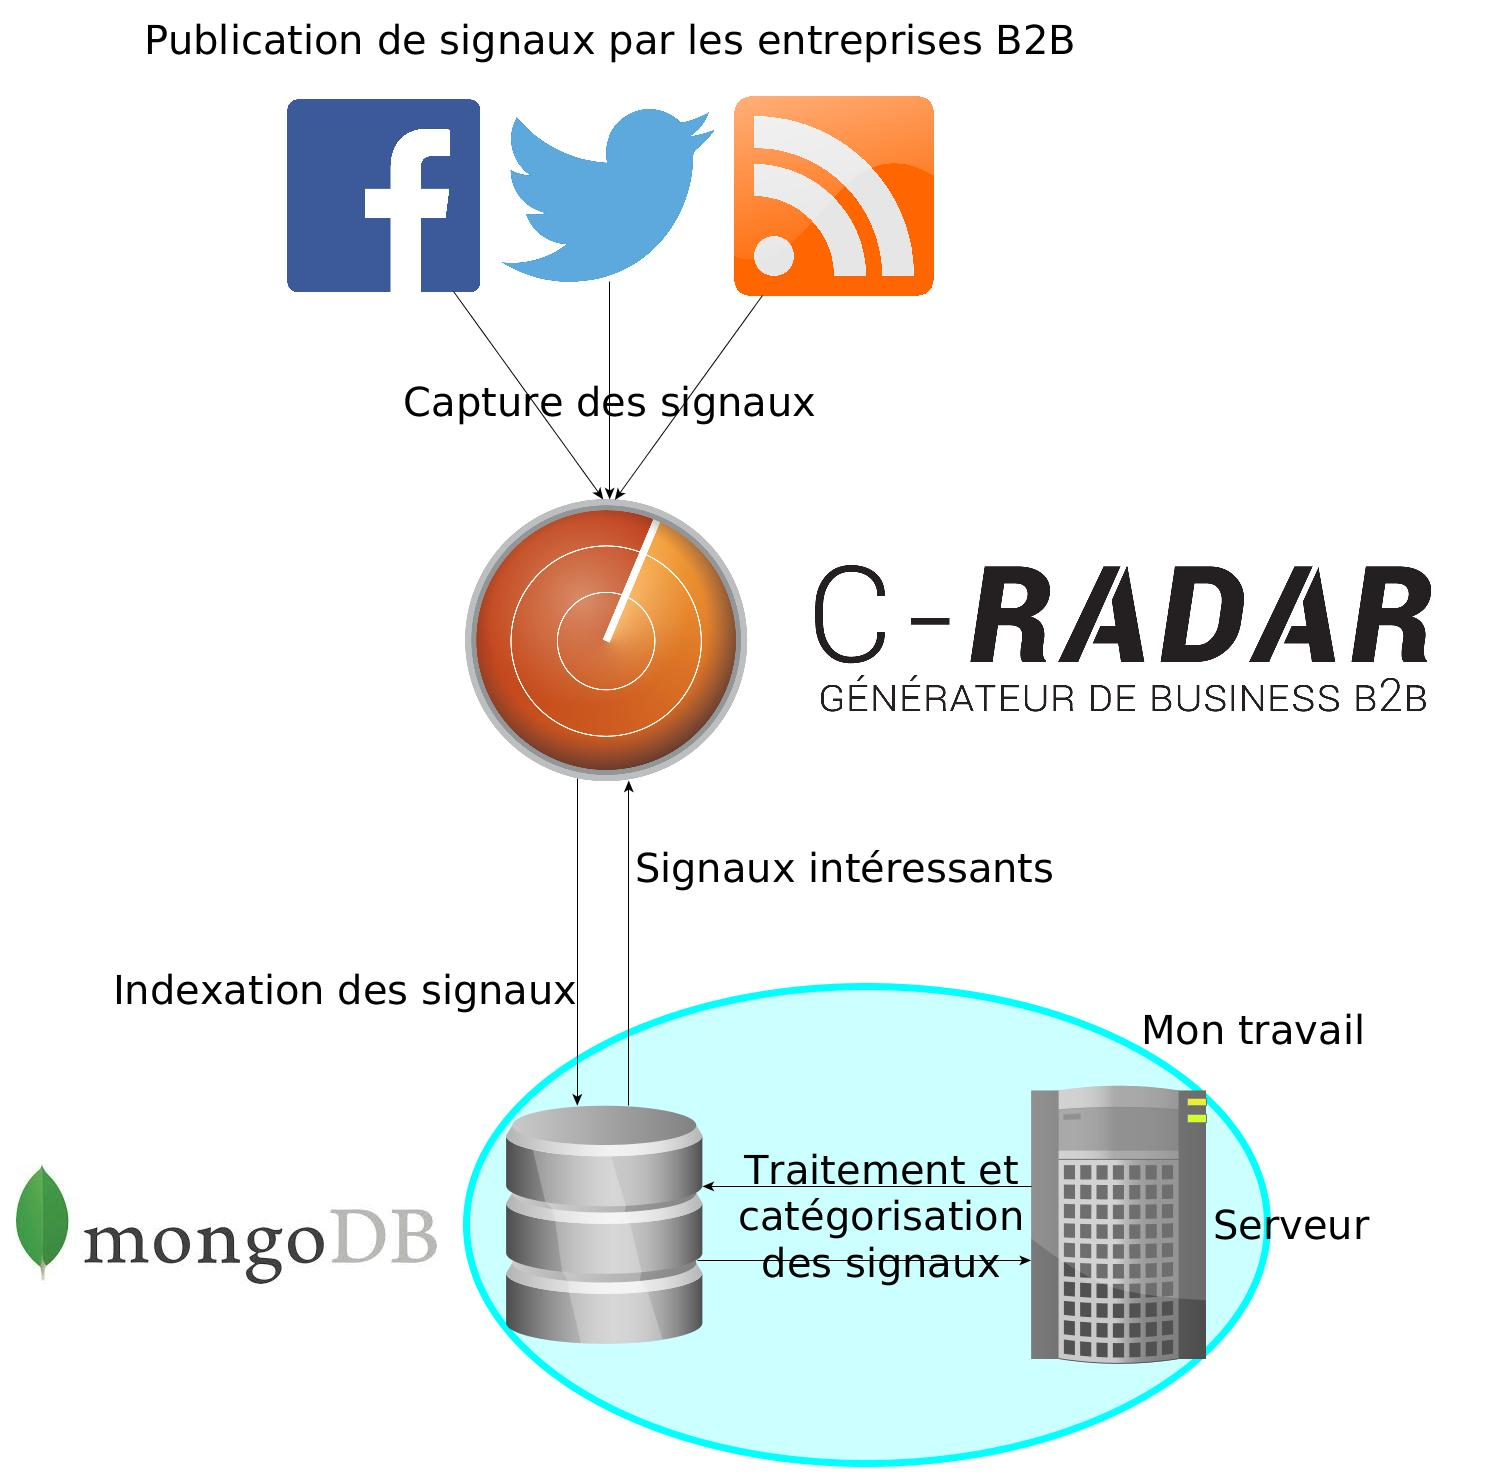
\includegraphics[width=0.75\textwidth]{images/capture_process.jpg}
        \caption{Le fonctionnement générale de cette fonctionnalité.}
        \label{fig:capture_process}
    \end{figure}

    De l'offre d'emploi, à la participation à des salons, en passant par les nominations de personnel ainsi que les présentations des derniers produits ou encore des éventuelles levées de fonds ou investissements, la communication des entreprises n'est plus équivoque mais belle et bien ordonnée grâce à cette fonctionnalité. On peut désormais savoir quelles sont les derniers postes à pourvoir chez Orange, par exemple, ou encore les dernière nomination qui ont eu lieux à la Banque Postale.\\

    Le fonctionnement générale de cette fonctionnalité est le suivant (visible en figure \ref{fig:capture_process}) :
    \begin{enumerate}
        \item C-Radar capte tout les signaux émis par les entreprises sur les réseaux sociaux (Facebook et Twitter), dans les médias ou via des flux RSS. Ces signaux sont ensuite stocké dans une base de données Mongo.
        \item Une fois ces signaux capturés et stocké, il faut les traiter afin d'identifier l'intérêt potentiel de leur contenu.
    \end{enumerate}
    C'est sur ce second point que j'interviens.
% section la_fonctionnalit_de_c_radar (end)

\section{Ma mission chez Data Publica} % (fold)
\label{sec:ma_mission_chez_data_publica}
    Ma mission est de construire une chaîne de traitement automatique, un plugin Python, récupérant la liste des signaux émis par les entreprises en entrée depuis un point d'API, leur appliquer les traitements nécessaires afin de fournir, en sortie, la liste des signaux intéressants ainsi que leur catégories respectives.\\

    Il s'agit donc de construire une application, un plugin Python, capable de classifier un signal dans une catégorie par la seule connaissance de son contenu (éventuellement un titre). L'application traitera donc des documents textuels.\\
    Le travail se divise en deux étapes :
    \begin{enumerate}
        \item Appliquer une série de prétraitements sur le contenu des signaux afin de sélectionner les features jugés porteurs d'information. En effet, comme les données manipulées sont textuelles, il faut filtrer certaines chaînes de caractères considérées comme du bruit.
        \item Construire un classifieur à partir des features sélectionnés parmi les données que l'on juge porteur d'information.
    \end{enumerate}

    \subsection{Inscription dans le domaine du \textit{Big Data}}
        Les tâches qui découlent de ma mission, et notamment tout les prétraitements, sont directement liées à la discipline de la fouille de textes (\textit{Text Mining}) (et de l'\textit{Information Retrieval}) pour trouver des informations dans le contenu des signaux. Elles sont également liées à la discipline du traitement automatique du langage naturel (\textit{Natural Language Processing}). Enfin, la construction du classifieur automatique implique des compétences en \textit{Machine Learning}.\\

    \subsection{Synthèse du travail à réaliser}
        Si l'on devait résumer le travail à effectuer (visible en figure \ref{fig:capture_process}), on pourrait le synthétiser comme ceci : Construire une application (plugin Python), qui prend en entrée un signal émis par une entreprise et répond aux questions suivantes :
        \begin{enumerate}
            \item Ce signal a-t-il de l'intérêt ?
            \item Si oui, quel est le sujet du signal ? Parle -t-il d'une offre d'emploi, d'une nomination, d'une levée de fond, etc ?
        \end{enumerate}
        La figure \ref{fig:process} montre ce que l'application (le plugin Python) doit être capable de faire.

        \begin{figure}[h!]
            \centering
            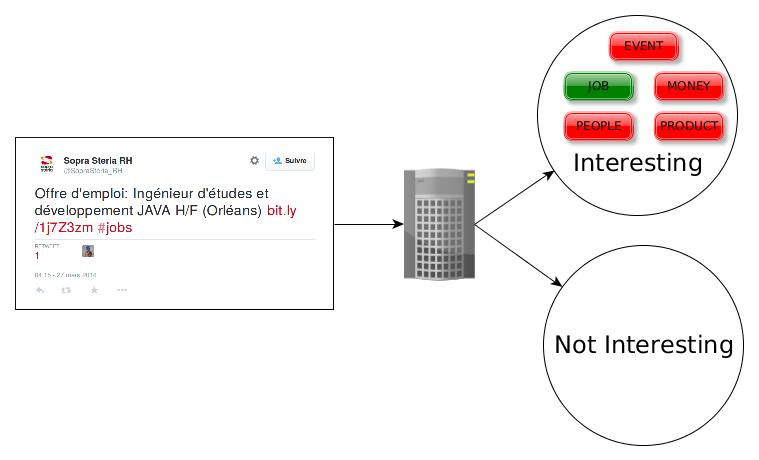
\includegraphics[width=\textwidth]{images/process.jpg}
            \caption{La tâche du plugin Python.}
            \label{fig:process}
        \end{figure}

\section{Présentation des signaux}
\label{sec:etat_bd}
    Les signaux sont des posts Facebook, des tweets ou bien des flux RSS publiés par des entreprises.

    \paragraph{Hypothèses de départ :}
        On considérera qu'un signal est intéressant si son contenu a pour sujet :
        \begin{itemize}
            \item Une offre d'emploi (ou un stage) à pourvoir au sein de l'entreprise qui l'a postée. Par la suite, on associera le tag \textit{JOB} à cette catégorie.
            \item Un évènement auquel l'entreprise participe (un salon par exemple). Par la suite, on associera le tag \textit{EVENT} à cette catégorie.
            \item Un produit que l'entreprise vient de présenter. Par la suite, on associera le tag \textit{PRODUCT} à cette catégorie.
            \item Une nomination d'un employé dans l'entreprise ou d'une entreprise vers une autre entreprise. Par la suite, on associera le tag \textit{PEOPLE} à cette catégorie.
            \item Une levée de fonds, un investissement, ou encore une déclaration de résultats ou de chiffre d'affaire.. Par la suite, on associera le tag \textit{MONEY} à cette catégorie.
        \end{itemize}

    \paragraph{Exemple de signal type pour chaque catégorie :}
        \begin{itemize}
            \item \textit{JOB} : \og Offre d'emploi: Ingénieur d'études et développement JAVA H/F (Orléans) http://t.co/LOvN8rLHIe \#jobs \fg
            \item \textit{EVENT} : \og  Fraispertuis sera présent dès demain jusqu'à dimanche inclus au salon \og Tourrissimo \fg de Strasbourg Parc des Expositions, Hall 21 Stand B40, venez rendre visite au capt'ain Fraisp ! \fg
            \item \textit{PRODUCT} : \og Découvrez quelques unes de nos réalisations de Pergola Biotempérée pour notre clientèle de Toulouse et sa région. Plus d'informations sur notre site www.pergola-biotemperee.com \fg
            \item \textit{PEOPLE} : \og Matthieu Frairot a été nommé Directeur Associé au sein de l'agence FullSIX France, l'agence marketin http://t.co/Z2ENeeWZmF \fg
            \item \textit{MONEY} : \og Keyrus : Publication des résultats annuels 2013. http://t.co/k4TPJ11fW4 \fg
        \end{itemize}

    \paragraph{État de l'ensemble des signaux :}
        Au 08/06/2015, seul 1426 signaux ont été validés manuellement avec potentiellement un tag (JOB, EVENT, PRODUCT, MONEY ou PEOPLE), dans le cas où le signal est intéressant.\\
        La proportion des classes de cet échantillon est mauvaise, c'est-à-dire que les données souffrent d'un fort déséquilibre entre classes : il y a beaucoup plus de signaux inintéressants qu'intéressants. Je n'avait donc pas assez d'exemples de signaux intéressants pour pouvoir considérer les éventuelles prédictions d'un classifieur construit sur la base de ces données comme correctes. Il est donc nécessaire d'en valider d'autres manuellement.

% section ma_mission_chez_data_publica (end)